\documentclass[12pt]{article}

% Paketi za ćirilicu i jezik
\usepackage[utf8]{inputenc}
\usepackage[T2A]{fontenc}
\usepackage[serbianc]{babel}
\usepackage{xcolor}
\usepackage{graphicx}
\usepackage{amsmath}
\usepackage{ntheorem}
\usepackage{caption}

% PAKET ZA KLIKABILNE LINKOVE (DODATO)
\usepackage[colorlinks=true, linkcolor=blue, urlcolor=red]{hyperref}

% Podešavanje okruženja na ćirilici
\newtheorem{definicija}{Дефиниција}
\newtheorem{teorema}{Теорема}
\newtheorem{lema}{Лема}

\title{Анализа рачунарског црва Stuxnet}
\author{Ђорђе Митровић \\ Индекс: 42/2025}
\date{\today}

\begin{document}

\maketitle

% Sadržaj na početku - sada je klikabilan!
\tableofcontents
\newpage

\section{Увод}
\textbf{Stuxnet} представља један од најсложенијих малициозних софтвера икада направљених. Његова примарна сврха била је саботажа индустријских контролних система (ICS). 


\section{Техничке карактеристике}
\subsection{Структура кода}

Црв је специфичан по томе што комбинује различите методе напада. Његове кључне компоненте укључују:

\begin{itemize}
    \item \textbf{LNK датотеке:} Коришћене за аутоматско извршавање кода са USB стикова.
    \item \textbf{Zero-day рањивости:} Чак четири до тада непозната безбедносна пропуста.
    \item \textbf{PLC rootkit:} Део кода који скрива присуство црва на индустријским контролерима.
\end{itemize}
\begin{description}
    \item[SCADA] Системи за надзор и контролу.
    \item[PLC] Програмабилни логички контролери.
\end{description}
Црв је користио чак четири \textit{zero-day} рањивости. Математички модел ширења:
\begin{equation}
P(t) = \frac{1}{1 + e^{-k(t-t_0)}}
\end{equation}

\section{Визуелни приказ и дефиниције}

\noindent
\begin{minipage}{0.45\textwidth}
    \centering
    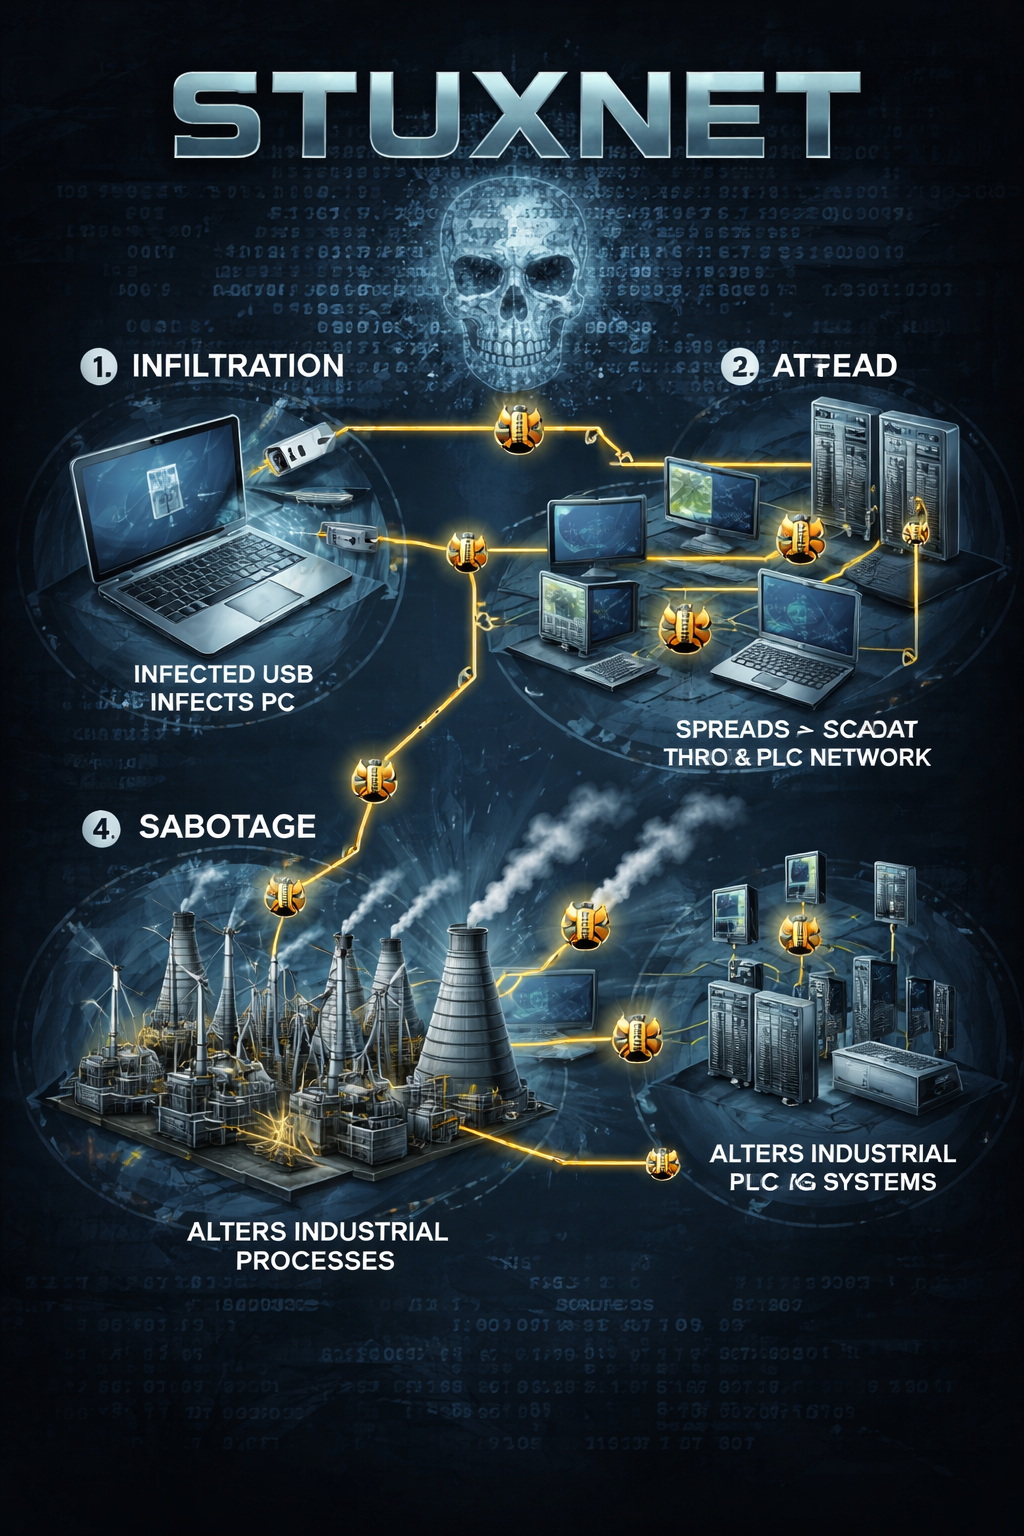
\includegraphics[width=\textwidth]{slike/stuxnet.png}
    \captionof{figure}{Симболични приказ Stuxnet-а}
\end{minipage}
\hfill
\begin{minipage}{0.5\textwidth}
    \begin{definicija}
    Сајбер-оружје је злонамерни код развијен у сврху наношења штете критичној инфраструктури.
    \end{definicija}

    \begin{lema}
    Сваки софтвер који утиче на \textit{PLC} може бити оружје.
    \end{lema}

    \begin{teorema}
    Ако је код потписан валидним сертификатом, вероватноћа је $V \approx 1$.
    \end{teorema}
\end{minipage}

\vspace{1cm} 

\section{Анализа података}
\begin{table}[h]
\centering
\begin{tabular}{|l|c|r|}
\hline
\textbf{Држава} & \textbf{Проценат инфекција} & \textbf{Тип циља} \\ \hline
Иран & 58.85\% & Нуклеарна постројења \\ \hline
Индонезија & 18.22\% & Енергетика \\ \hline
Индија & 8.31\% & Индустрија \\ \hline
\end{tabular}
\caption{Дистрибуција инфекције Stuxnet црвом}
\end{table}

\section{Закључак}
Stuxnet је променио начин на који посматрамо \textcolor{red}{модерно ратовање}.
\begin{enumerate}
    \item \textbf{Напад на хардвер:} Физичка штета путем софтвера.
    \item \textit{Air-gap} изолација није апсолутна заштита.
    \item Употреба украдених дигиталних потписа.
\end{enumerate}

\end{document}